\documentclass[../main.tex]{subfiles}
\graphicspath{{\subfix{../figures/}}}

\begin{document}
\section{接口隔离原则(ISP)}
Interface Segregation Principle

\noindent 接口隔离原则指的是:使用多个专门的细粒度接口比总使用单一的粗粒度接口要好.
换言之,从一个客户端类的角度来讲:一个类对另外一个类的依赖应当是建立在最小的接口上.

\textbf{角色的合理划分}: 可以将接口理解为一个类所具有的公有方法的集合.接口的划分就直接带来类型的划分.
 一个接口相当于剧本中的一种角色,而此角色在一个舞台上由哪一个演员来演则相当于接口的实现.因此,一个接口应当简单地代表一个角色,而不是多个.我们将这种角色划分的原则叫做角色隔离原则.

 \textbf{接口污染}:过于臃肿的接口是对接口的污染。
准确而恰当地划分角色以及角色所对应的接口,是面向对象设计的一个重要组成部分。
将没有关系的接口合并在一起,形成一个臃肿的大接口,是对角色和接口的污染。

\textbf{定制服务}也是一个重要的设计原则。含义:如果客户端仅仅需要某一些方法的话,就应当向客户端提供这些需要的方法,而不要提供其不需要的方法。
这样做的效果:
\begin{itemize}
  \item 很整洁(设计师需要花较多时间在分析和划分这些接口)
  \item 系统的可维护性。(尽量不提供public接口)
\end{itemize}
%
\subsection{全文搜索引擎的系统设计}
一个动态的资料网站将大量的文件资料存储在文件中或关系数据库里面,用户可以通过输入一个和数个关键词进行全网站的全文搜索。这个搜索引擎需要维护一个索引库,索引库以文本文件方式存于文件系统中。在源数据被修改,删除或者增加时,搜索引擎要做相应的动作,以保证引擎的索引文件也被相应的更新。

首先,下面所示为一个不好的解决方案。一个叫做BadExample的接口负责所有的操作,从提供搜索功能到建立索引功能,甚至包括搜索结果集合的功能均在一个接口内提供。
如下图所示:
\begin{figure}[H]
  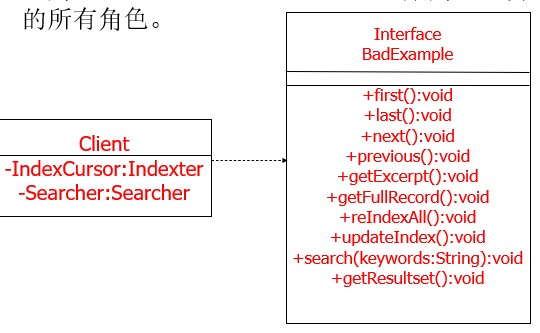
\includegraphics[width=0.55\textwidth]{11_1.jpg}
\end{figure}
这个解决方案违反了角色风格原则,把不同功能的接口放在一起,由一个接口给出包括搜索器角色,索引生成器以及搜索结果集角色在内的所有角色。

\textbf{角色的分割}:
\begin{figure}[H]
  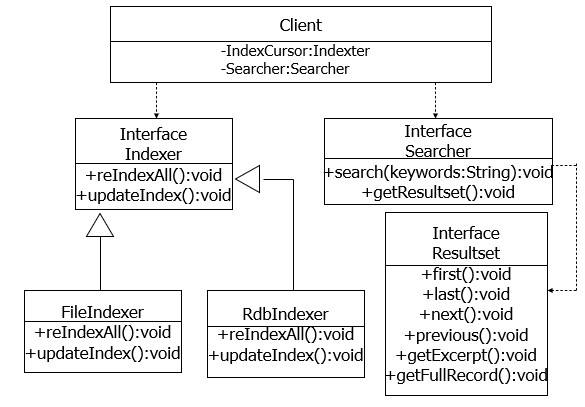
\includegraphics[width=0.55\textwidth]{11_2.jpg}
\end{figure}
由图中可看出,搜索引擎的功能被分割成三个角色:
搜索器角色,
索引生成器角色,
搜索结果集角色.

以``2''为例,由于索引生成因数据的格式不同而不同,故分为RdbIndexer和FileIndexer两种实现。 FileIndexer类代表对诸如*.txt,*.html,*.doc以及*.pdf等文件类型的数据生成全文索引,而RdbIndexer则针对关系数据库的数据进行全文索引生成。这两个实现扮演的同为索引生成器角色,就好像扮演同样角色的两个不同演员一样。

搜索器角色则是与索引生成器角色完全不同的角色,它提供用户全文搜索功能。用户传进一些关键字,搜索器角色则返回一个ResultSet。
搜索结果集角色就是ResultSet。它给用户提供对集合进行迭代走访的功能,如first()将光标移到集合的第一个元素;last()将光标移到结婚的最后一个元素;next()将光标移到集合的下一个元素;previous()将光标移到集合的前一个元素;而getExcerpt()则返回当前记录的摘要;而getFullRecord()则将记录的全文返回.
\end{document}
